\documentclass[12pt, a4paper]{article}
\usepackage[utf8]{inputenc}
\usepackage{amsmath}
\usepackage{amsfonts}
\usepackage{amsthm}
\usepackage{array}
\usepackage{graphicx}
\usepackage{parskip}
\usepackage[pdfencoding=auto]{hyperref}
\usepackage{fancyhdr}
\usepackage{lastpage}
\usepackage{tikz}
\usepackage{float}
\usepackage{listings}
\usepackage{color}
\usepackage{caption}
\usepackage{authblk}
\usepackage[acronym]{glossaries}
\usepackage[nottoc]{tocbibind}
\usepackage[cache=false]{minted}
\usemintedstyle{default}
\newminted{haskell}{frame=lines,framerule=2pt}
\newminted{R}{frame=lines,framerule=2pt}
\graphicspath{{./images/}}

\tikzstyle{bag} = [align=center]

\title{%
      Homework 6\\
      Network Dynamics Analysis\\
}
\author{Juan Pablo Royo Sales \& Francesc Roy Campderrós}
\affil{Universitat Politècnica de Catalunya}
\date\today

\pagestyle{fancy}
\fancyhf{}
\fancyhead[C]{}
\fancyhead[R]{UPC MIRI}
\fancyhead[L]{CSN - Homework 6}
\fancyfoot[L,C]{}
\fancyfoot[R]{Page \thepage{} of \pageref{LastPage}}
\setlength{\headheight}{15pt}
\renewcommand{\headrulewidth}{0.4pt}
\renewcommand{\footrulewidth}{0.4pt}

\newacronym{netdyn}{Network Dynamics}{Network Dynamics}
\newacronym{degdist}{Degree Distribution}{Degree Distribution}
\newacronym{growdeg}{Time Growth Degree}{Growth of Vertex Degree over time}
\newacronym{indegree}{Incomming Degree}{Incomming Degree Language Set}
\newacronym{dispp}{Displaced Poisson}{Displaced Poisson Model}
\newacronym{dispg}{Displaced Geometric}{Displaced Geometric Model}
\newacronym{zeta2}{Zeta-Gamma-2}{Zeta Model with fixed Gamma with value 2}
\newacronym{zeta}{Zeta}{Zeta Model}
\newacronym{zetar}{Right-Truncated Zeta}{Right-Truncated Zeta Model}
\newacronym{aic}{Akaike}{Akaike Information Criterion}
\newacronym{alt}{Altmann}{Altmann Model}

\begin{document}

\maketitle

\tableofcontents

\section{Introduction}
In this homework we have analyzed \acrfull{netdyn} on different models proposed for this work.
The main goal of this work is to identify the best model which fit on both aspects of \acrshort{netdyn}, 

\section{Results}
\subsection{Degree Distribution Analysis}
\subsubsection{Growth + Preferential Attachment}

\begin{table}[H]
    \centering
    \begin{tabular}{l r}
        Parameter & Value\\
        \hline              
        M & 200002\\
        N & 100002\\
        MAX & 1105\\
        M/N & 1.99\\
        N/M & 0.50\\
        MP & 37263.76\\
        C & 205119.83
    \end{tabular}
    \caption{Data Analysis over Growth + Pref Attachment}
    \label{table:grow_pref_att_1}
\end{table}

\begin{table}[H]
    \centering
    \begin{tabular}{l r}
        Distribution & Estimation\\
        \hline
        Displaced Poisson & 1.59\\
        Displaced Geometric & 0.50\\
        Zeta Gamma & 2.29\\ 
        Zeta Truncated & 103002\\
    \end{tabular}
    \caption{Estimation of Parameters: Growth + Pref Attachment}
    \label{table:grow_pref_att_2}
\end{table}

\begin{table}[H]
    \centering
    \begin{tabular}{l r}
        Distribution & AIC Value\\
        \hline
        Displaced Poisson & 253849.2\\
        Displaced Geometric & 33974.32\\
        Zeta Gamma 3 & 17100.8\\
        \textbf{Zeta Gamma} & \textbf{0}\\ 
        Zeta Truncated & 1.966677\\
    \end{tabular}
    \caption{AIC Selection: Growth + Pref Attachment}
    \label{table:grow_pref_att_3}
\end{table}

\begin{minipage}[t]{\linewidth}
    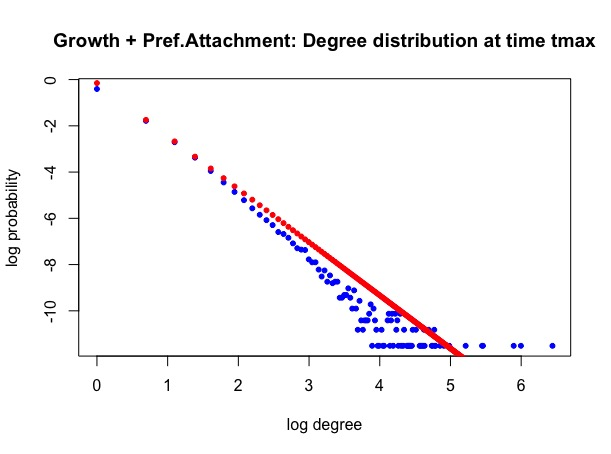
\includegraphics[width=\textwidth]{degree_tmax_grow_pref_att}
    \captionsetup{type=figure}
    \captionof{figure}{Degree $t_{max}$ Growth + Pref Att with Zeta $\Gamma = 3$}
    \label{fig:degree_tmax_grow_pref_att}
  \end{minipage}

\subsubsection{Growth + Random Attachment}

\begin{table}[H]
    \centering
    \begin{tabular}{l r}
        Parameter & Value\\
        \hline              
        M & 200002\\
        N & 100002\\
        MAX & 16\\
        M/N & 1.99\\
        N/M & 0.50\\
        MP & 50775.59\\
        C & 136242.14
    \end{tabular}
    \caption{Data Analysis over Growth + Random Attachment}
    \label{table:grow_ran_att_1}
\end{table}

\begin{table}[H]
    \centering
    \begin{tabular}{l r}
        Distribution & Estimation\\
        \hline
        Displaced Poisson & 1.59\\
        Displaced Geometric & 0.50\\
        Zeta Gamma & 2.07\\ 
        Zeta Truncated & 103002\\
    \end{tabular}
    \caption{Estimation of Parameters: Growth + Random Attachment}
    \label{table:grow_ran_att_2}
\end{table}

\begin{table}[H]
    \centering
    \begin{tabular}{l r}
        Distribution & AIC Value\\
        \hline
        Displaced Poisson & 82119.5\\
        \textbf{Displaced Geometric} & \textbf{0}\\
        Zeta Gamma 3 & 64197.51\\
        Zeta Gamma & 24921.01\\ 
        Zeta Truncated & 24922.54\\
    \end{tabular}
    \caption{AIC Selection: Growth + Random Attachment}
    \label{table:grow_ran_att_3}
\end{table}

\begin{minipage}[t]{\linewidth}
    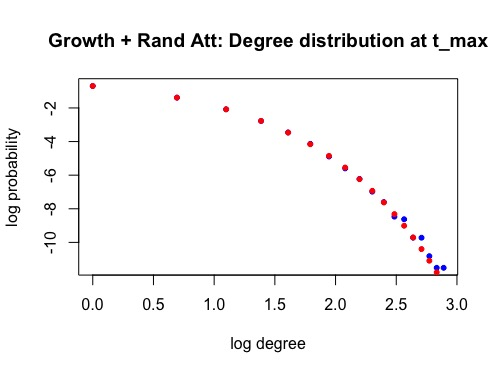
\includegraphics[width=\textwidth]{degree_tmax_grow_random_att}
    \captionsetup{type=figure}
    \captionof{figure}{Degree $t_{max}$ Growth + Pref Att with Displaced Geometric}
    \label{fig:degree_tmax_grow_pref_att}
  \end{minipage}

\subsection{Time Growth Degree Analysis}
\subsubsection{Growth + Preferential Attachment}
\begin{minipage}[t]{\linewidth}
    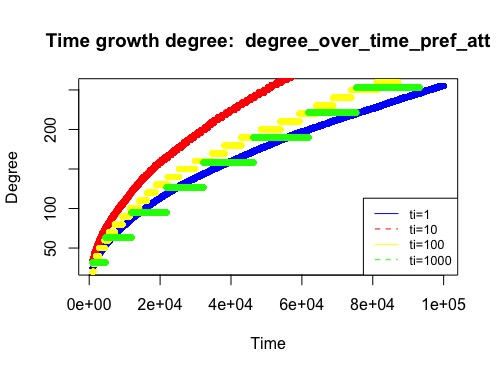
\includegraphics[width=\textwidth]{time_growth_degree_pref_att}
    \captionsetup{type=figure}
    \captionof{figure}{Time Growth Degree: Growth + Pref Att}
    \label{fig:time_growth_degree_pref_att}
  \end{minipage}
\subsubsection{Growth + Random Attachment}


\section{Discussion and Methods}
fafdsaf

\section{Conclusions}
fadsfasdf

\end{document}

